\thispagestyle{cackithitoannone}
\pagestyle{cackithitoan}
\everymath{\color{cackithi}}
\graphicspath{{../cackithi/pic/}}
\blfootnote{{\color[named]{cackithi}$^1$Trường Đại học Mỏ--Địa chất.}}
\begingroup
\AddToShipoutPicture*{\put(0,616){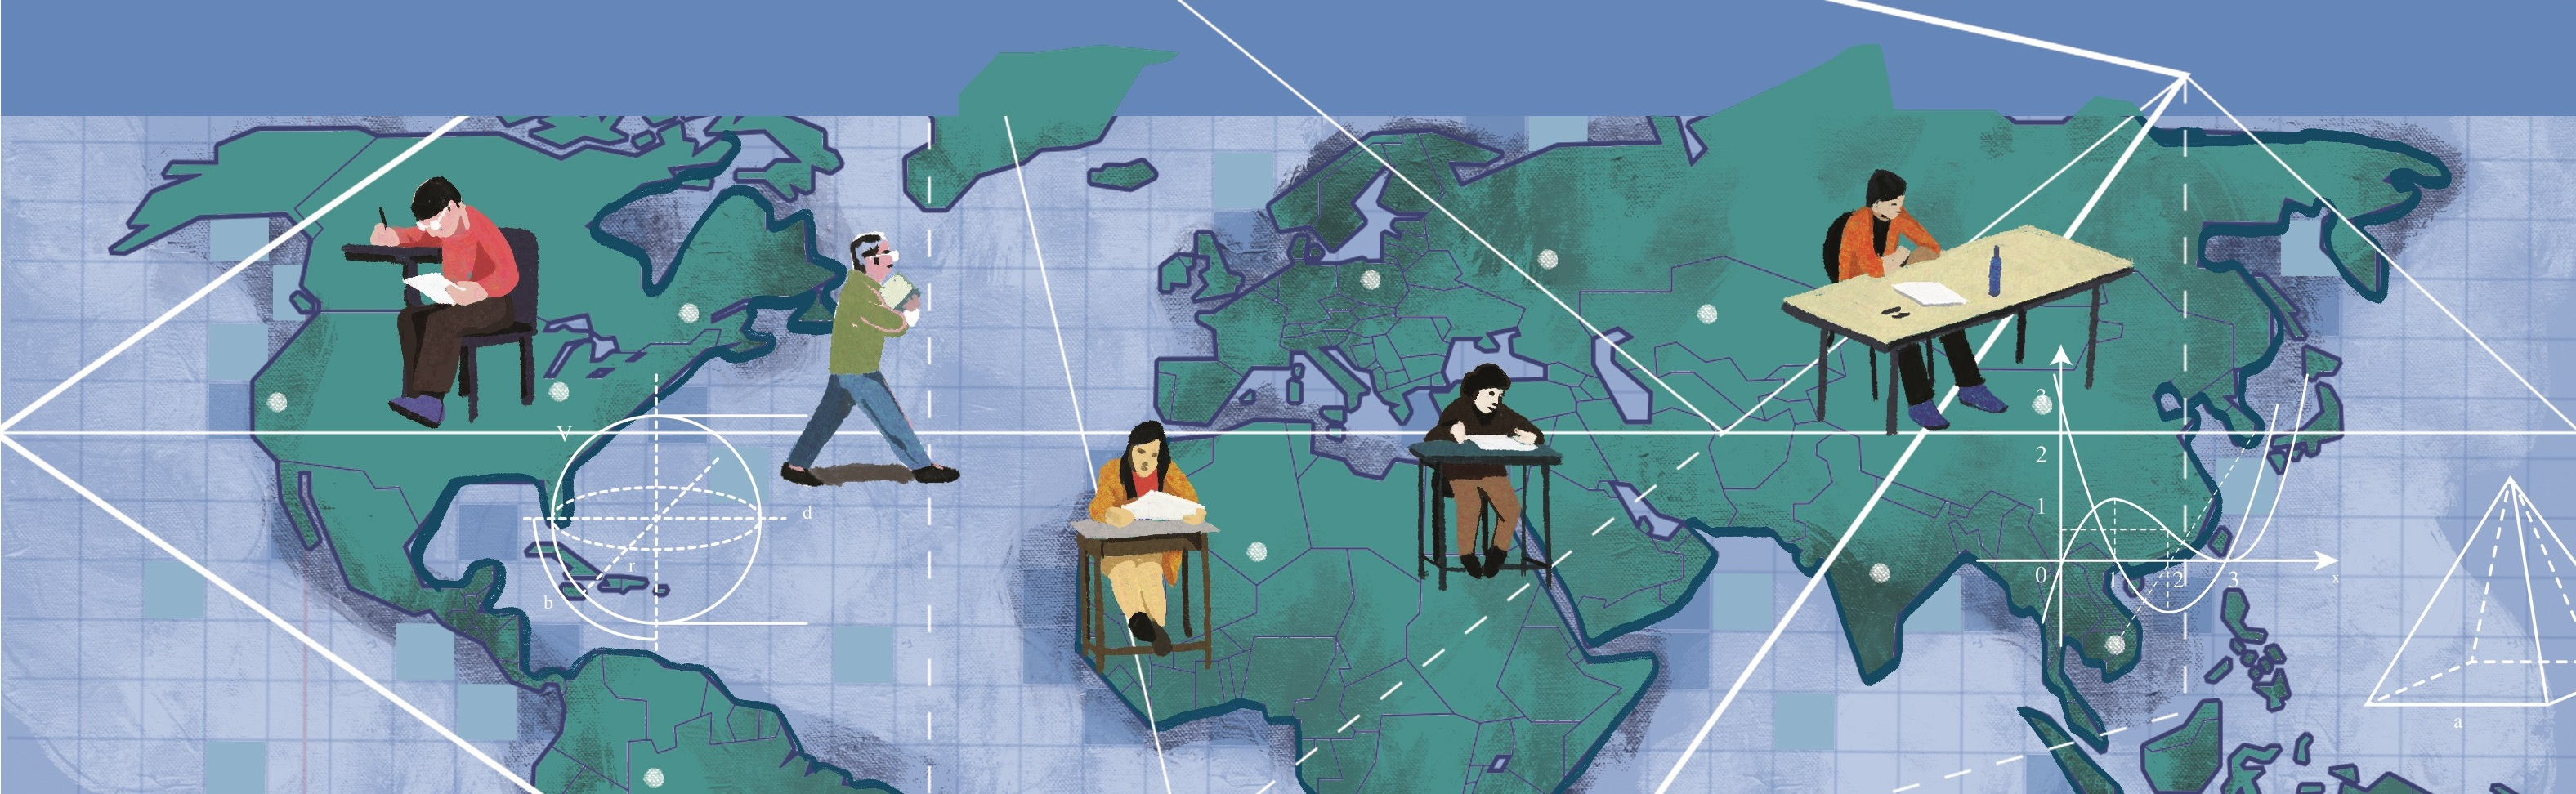
\includegraphics[width=19.3cm]{../bannercackithi}}} 
\AddToShipoutPicture*{\put(64,526){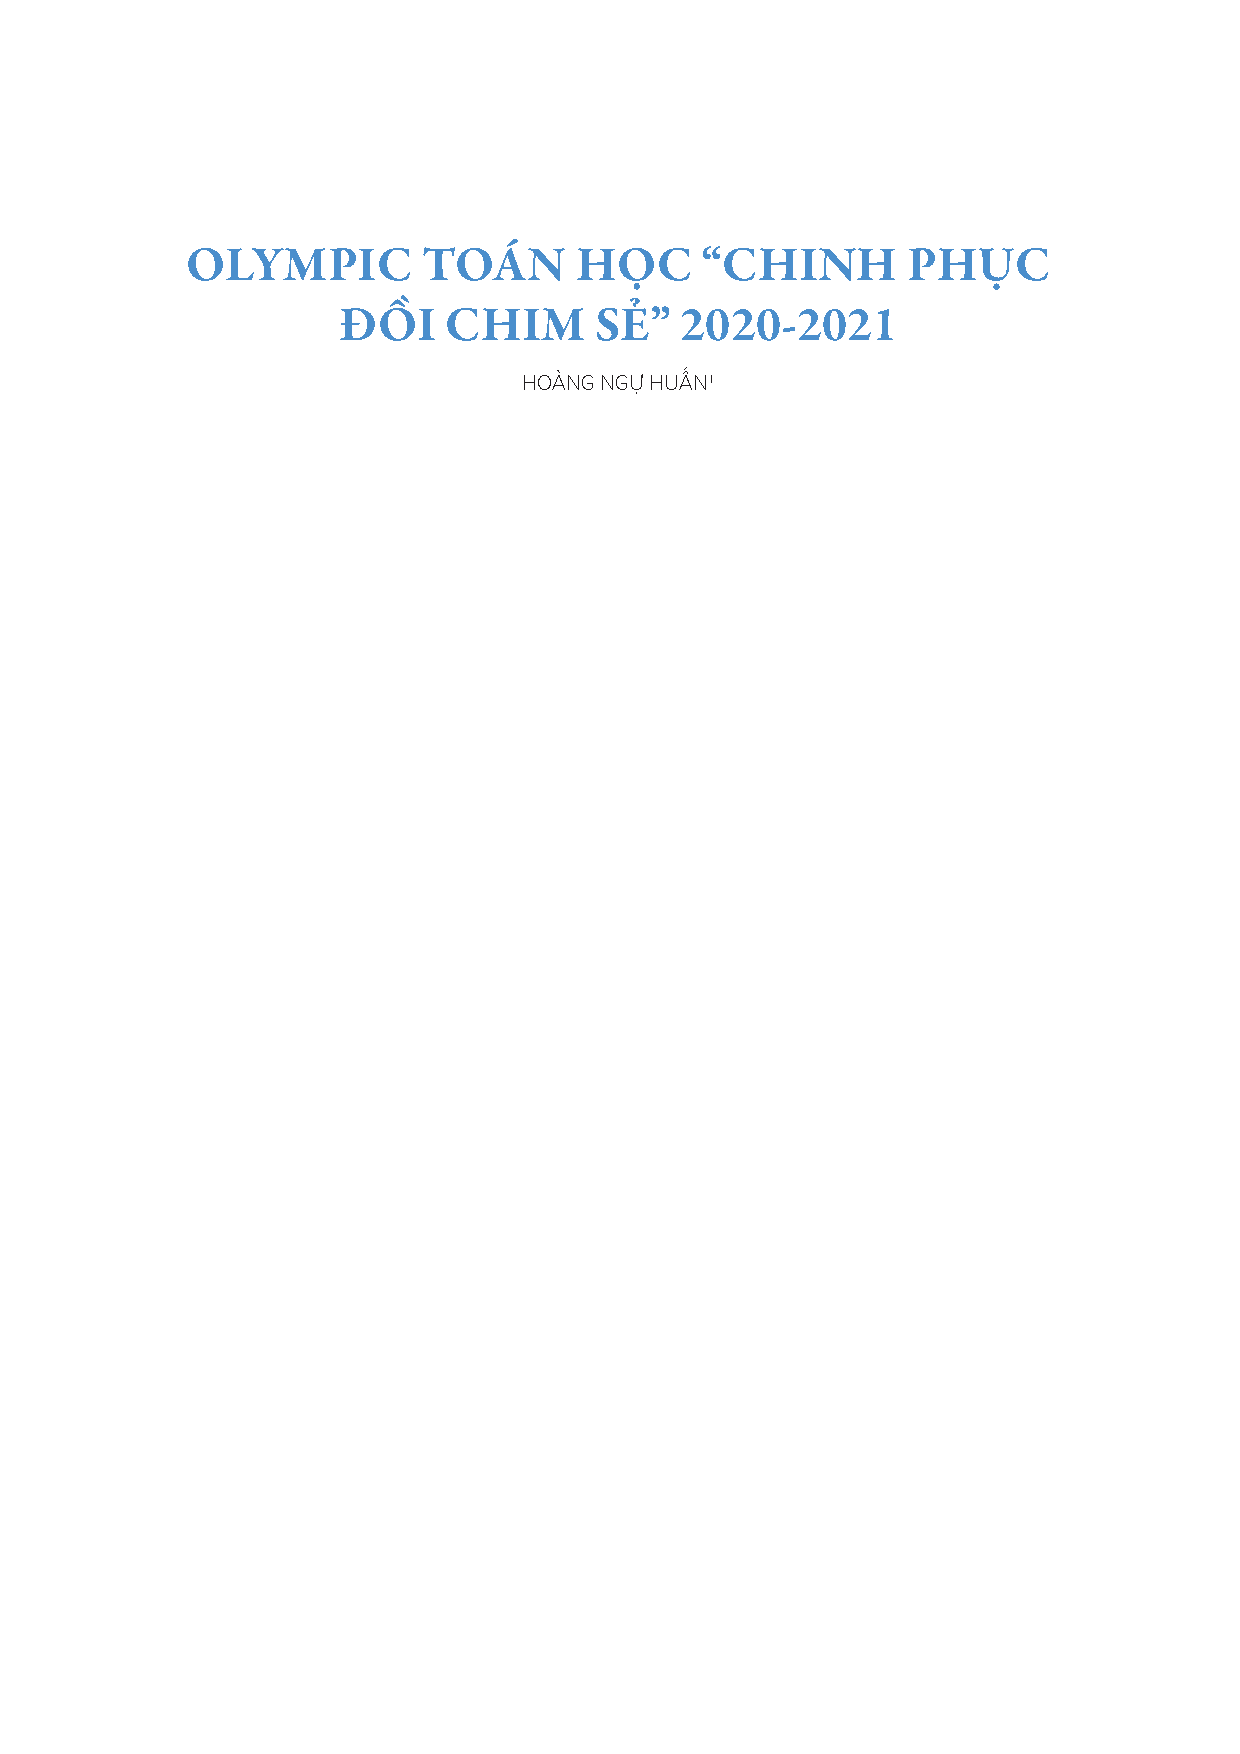
\includegraphics[scale=1]{../tieude3.pdf}}}
\centering
\endgroup
\vspace*{180pt}

\begin{multicols}{2}
	Xin được giới thiệu với bạn đọc về kỳ thi ``chinh phục đồi chim sẻ". Đây là kỳ thi do Trường đại học tổng hợp Moscow và nhà xuất bản thanh niên Moscow cùng phối hợp tổ chức từ năm $2005$ nhằm tuyển chọn sinh viên cho trường Đại học tổng hợp Moscow. Xin được nói thêm Trường Đại học tổng hợp Moscow là trường đại học lâu đời nhất và cũng là trường đại học nổi tiếng nhất nước Nga. Nơi đây đã đào tạo ra rất nhiều nhà khoa học danh tiếng. Thi đỗ vào trường là niềm mơ ước của rất nhiều học sinh Nga. Tham gia kỳ thi này là học sinh các lớp từ $9$ tới $11$. Trong đó có kỳ thi riêng dành cho lớp $11$ và cho các bạn lớp $9$ và $10$. Năm $2009$ có $500$ bạn học sinh đã được giải thưởng kỳ thi này và khoảng $400$ bạn đã trở thành sinh viên của trường. Sau đây là bài kiểm tra của năm $2021$.
	\vskip 0.1cm
	Kỳ thi ``Chinh phục đồi chim sẻ" năm học $2020/2021$ gồm hai vòng và đều tiến hành thi online. Vòng tuyển loại (diễn ra vào tháng $11-12$ năm $2020$) kéo dài $24$h gồm hai vòng nhỏ hơn: vòng loại có $6$ bài toán và kéo dài $3$ giờ, phần sáng tạo gồm $3$ bài toán và cần phải gửi lời giải trong khoảng thời gian còn lại. Vượt qua vòng tuyển loại, các bạn trẻ sẽ được tham gia vào vòng chung kết diễn ra vào tháng $4$ năm $2021$.
	\vskip 0.1cm
	\textbf{\color{cackithi}Vòng loại}
	\vskip 0.1cm
	\textit{Mỗi học sinh sẽ nhận được danh sách các bài toán riêng khác biệt. Sau đây là một ví dụ về sáu bài toán của vòng loại.}
	\vskip 0.1cm
	$\pmb{1.}$ Giải bất phương trình
	\begin{align*}
		\dfrac{{\sqrt {x + 5}  - x - 3}}{{{x^2} - 15x + 54}} \ge 0
	\end{align*}
	Trong đó hãy tìm số lượng nghiệm nguyên của bất phương trình trên.
	\vskip 0.1cm
	$\pmb{2.}$ Giải phương trình $\cos 2x + \cos 6x + 2\sin^2 x = 1$.
	\vskip 0.1cm
	Trong đó hãy chỉ ra tổng các nghiệm thuộc đoạn $\left[ {\dfrac{{5\pi }}{6};\;\pi } \right]$, làm tròn tới hai chữ số sau dấu phảy.
	\vskip 0.1cm
	$\pmb{3.}$ Từ điểm $M$ nằm trong tam giác $ABC$ hạ các đường vuông góc xuống các cạnh $BC$, $AC$, $AB$. Các đường vuông góc này có độ dài tương ứng là $k$, $l$ và $m$. Tìm diện tích của tam giác $ABC$, biết rằng $\angle CAB = \alpha$ và  $\angle ABC = \beta$. Nếu kết quả thu được không là số nguyên, hãy làm tròn nó tới số nguyên gần nhất.
	\vskip 0.1cm
	Cho biết các giá trị số là:  $\alpha = \dfrac{\pi}{6}, \beta = \dfrac{\pi}{4},k=3  ,l=2  ,m=4$.
	\vskip 0.1cm 
	$\pmb{4.}$ Giải hệ sau
	\begin{align*}
		\begin{cases}
			x^3 + 3y^2 = 11,\\
			x^2y + xy^2 = 6.
		\end{cases}
	\end{align*}
	Với mỗi nghiệm $(x,y)$ của hệ, hãy tính giá trị của biểu thức $\dfrac{x}{y}$; sau đó tìm giá trị nhỏ nhất trong các giá trị thu được -- lấy xấp xỉ tới hai chữ số sau dấu phảy.
	\vskip 0.1cm
	$\pmb{5.}$ Có hai hợp kim. Hợp kim thứ nhất chứa $p\%$ tạp chất, hợp kim thứ hai chứa $q\%$ hợp chất. Hỏi rằng cần phải nung chảy hai hợp kim theo một tỷ lệ nào để thu được một hợp kim mới chứa $r\%$ tạp chất. Trong đáp án khi tính xấp xỉ tỷ lệ khối lượng của hợp kim thứ nhất với khối lượng của hợp kim thứ hai thì làm tròn tới hai chữ số sau dấu phảy.
	\vskip 0.1cm
	Các dữ liệu số: $p = 70, q = 5, r = 40$.
	\vskip 0.1cm
	$\pmb{6.}$ Hãy tìm tất cả các số nguyên $a$ có giá trị tuyệt đối không vượt quá $15$ sao cho bất đẳng thức 
	\begin{align*}
		\dfrac{{4x - a - 4}}{{6x + a - 12}} \le 0
	\end{align*}
	thỏa mãn với mọi $x$ thuộc khoảng  $[2,3]$. Sau đó hãy tính tổng tất cả các giá trị $a$ vừa tìm được.
	\vskip 0.1cm
	\textbf{\color{cackithi}Vòng tuyển chọn (phần sáng tạo)}
	\vskip 0.1cm
	$\pmb{7.}$ Tìm tất cả các số tự nhiên $n$ không vượt quá $100$ sao cho tổng ${1^2} + {2^2} + {3^2} + ... + {n^2}$  chia hết cho $50$.
	\vskip 0.1cm
	Với những giá trị $n$ vừa tìm được, hãy sắp xếp chúng theo thứ tự tăng dần:  ${n_1} < {n_2} < ... < {n_k}$. Từ đó hãy cho biết $n_{k-2}$ là số nào?
	\vskip 0.1cm
	$\pmb{8.}$ Cho trước một đường tròn, trong tất cả các tam giác nội tiếp đường tròn có tổng bình phương của các góc là $\alpha^2 + \beta^2 = \gamma^2 = \dfrac{\pi^2}{2}$ (các góc  $\alpha$,  $\beta$, $\gamma$ được tính bằng radian) hãy tìm tất cả các tam giác có diện tích lớn nhất.
	\vskip 0.1cm
	Với mỗi tam giác tìm được, hãy tìm giá trị nhỏ nhất của tích các cặp góc. Giá trị nhỏ nhất được làm tròn tới hai chữ số sau dấu phảy. 
	\vskip 0.1cm
	$\pmb{9.}$ Hãy tìm tất cả các cặp số dương $x$, $y$ thỏa mãn đẳng thức
	\begin{align*}
		&\dfrac{{4{x^2}y + 6{x^2} + 2xy - 4x}}{{3x - y - 2}} \\
		&+ \sin \left( {\dfrac{{3{x^2} + xy + x - y - 2}}{{3x - y - 2}}} \right)\\
		= &\,2xy + {y^2} + \dfrac{{{x^2}}}{{{y^2}}} + \dfrac{{2x}}{y} + \dfrac{{2xy({x^2} + {y^2})}}{{{{(3x - y - 2)}^2}}} + \\
		&+ \dfrac{1}{{{{(x + y)}^2}}}\left( {x^2}\sin \dfrac{{{{(x + y)}^2}}}{x}\right. \\
		&\left.+ {y^2}\sin \dfrac{{{{(x + y)}^2}}}{{{y^2}}} + 2xy\sin \dfrac{{{{(x + y)}^2}}}{{3x - y - 2}} \right).
	\end{align*}
	Trong đáp án hãy viết tổng $x^2 + y^2$ của tất cả các nghiệm  $(x,y)$. Kết quả được làm tròn tới hai chữ số sau dấu phảy. 
	\vskip 0.1cm
	\textbf{\color{cackithi}Vòng chung kết}
	\vskip 0.1cm
	\textbf{\color{cackithi}Đề $\pmb{1}$}
	\vskip 0.1cm
	$\pmb{10.}$ Viết các số tự nhiên bắt đầu từ $20$ thành một dòng: $20212223\ldots$ Hỏi rằng trong dãy kỹ tự thu được, chữ số nào đứng ở vị trí $2021$?
	\vskip 0.1cm
	$\pmb{11.}$ Hãy tìm tất cả các giá trị của $a$ sao cho phương trình
	\begin{align*}
		|x| \!-\! \arcsin x \!+\! b \!\cdot\! (\arccos x\, \!+\! |x| \!-\! 1) \!+\! a \!=\! 0
	\end{align*}
	có ít nhât một nghiệm với mọi giá trị của $b$.
	\vskip 0.1cm
	$\pmb{12.}$ Phương trình sau có bao nhiêu nghiệm
	\begin{align*}
		{2^{\lg ({x^2} - 3)}} = \lg {2^{{x^2} - 2}}?
	\end{align*}
	$\pmb{13.}$ Giải hệ sau
	\begin{align*}
		\begin{cases}
			2x - 3y + \dfrac{1}{xy} = 6,\\
			3z - 6x + \dfrac{1}{xz} = 2,\\
			6y - 2z + \dfrac{1}{yz} = 3.
		\end{cases}
	\end{align*}
	$\pmb{14.}$ Gấp một tờ giấy hình vuông có diện tích là $17$ theo đường thẳng đi qua tâm. Sau đó dính các mảnh lại với nhau. Hãy tìm diện tích lớn nhất trong các hình có thể tạo được.
	\vskip 0.1cm
	Trong khuôn khổ có hạn của bài báo, chúng tôi chỉ trình bày lời giải chi tiết đối với một số bài chọn lọc.  
	\vskip 0.1cm 
	\textbf{\color{cackithi}Đáp án và lời giải}
	\vskip 0.1cm
	\textbf{\color{cackithi}Vòng loại}
	\vskip 0.1cm
	$\pmb{1.}$ Đáp án: $7$.
	\vskip 0.1cm
	$\pmb{2.}$ Đáp án: $2{,}88$ (giá trị chính xác: $\dfrac{11\pi}{12}$).
	\vskip 0.1cm
	$\pmb{3.}$ Đáp án: $67$.
	\vskip 0.1cm
	$\pmb{4.}$ Đáp án: $-1{,}31$ (giá trị chính xác:  $-\dfrac{1+ \sqrt{217}}{12}$).
	\vskip 0.1cm
	$\pmb{5.}$ Đáp án: $1{,}17$ (giá trị chính xác:  $\dfrac{7}{6}$).
	\vskip 0.1cm
	$\pmb{6.}$ Đáp án:  $-7$.
	\vskip 0.1cm
	\textbf{\color{cackithi}Vòng tuyển chọn (phần sáng tạo)}
	\vskip 0.1cm
	$\pmb{7.}$ Đáp án: $87$.
	\vskip 0.1cm
	$\pmb{8.}$ Đáp án: $0{,}27$ (giá trị chính xác: $\dfrac{\pi^2}{36}$).
	\vskip 0.1cm
	$\pmb{9.}$ Đáp án: $4{,}33$ ($x = \dfrac{9 + \sqrt{17}}{8}$, $y = \dfrac{1+ \sqrt{17}}{4}$ và  $x^2 + y^2 = \dfrac{85 + 13\sqrt{17}}{32} \approx 4{,}33$).
	\vskip 0.1cm
	\textbf{\color{cackithi}Vòng chung kết}
	\vskip 0.1cm
	\textbf{\color{cackithi}Đề $\pmb{1}$}
	\vskip 0.1cm
	$\pmb{10.}$ Đáp án: $7$.
	\vskip 0.1cm 
	$\pmb{11.}$ Đáp án:  $\dfrac{\pi}{2} -1$.
	\vskip 0.1cm 
	\textit{Lời giải}. Khi  $b = -1$, phương trình có dạng $|x| - \arcsin x - \arccos x - |x| + 1 + a = 0$. Với $x \in [-1;1]$ phương trình tương đương với $1 + a - \dfrac{\pi}{2} = 0$. Như vậy, khi $b = -1$  nghiệm chỉ tồn tại khi $a = \dfrac{\pi}{2} - 1$.
	\vskip 0.1cm
	Mặt khác, khi $a = \dfrac{\pi}{2} -1$ phương trình $|x| - \arcsin x + b \cdot (\arccos x\, + |x| - 1) + \dfrac{\pi }{2} - 1 = 0$ có nghiệm $x =1$ với bất kỳ giá trị nào của $b$.
	\vskip 0.1cm
	\textit{Chú thích.} Các bạn thí sinh có nhiều lời giải không đúng vì dựa trên suy luận sau: câu văn từ điều kiện của bài toán ``với mọi giá trị của $b$ có ít nhất một nghiệm" thì bị hiểu nhầm là ``có cùng một nghiệm với mọi trí trị của $b$" (Đây là một bài toán khác, đơn giản hơn mặc dù đáp áp của nó trùng với đáp án của bài toán đã cho). 
	\vskip 0.1cm
	$\pmb{12.}$ Đáp án: $4$.
	\vskip 0.1cm 
	\textit{Lời giải.} Phương trình được biến đổi về dạng 
	\begin{align*}
		{t^\alpha } = \alpha (t + 1),
	\end{align*}
	với $\alpha  = \lg 2 \in (0,1)$, $t = {x^2} - 3 > 0$.
	\vskip 0.1cm
	Vì vế trái của phương trình $f\left( t \right) = {t^\alpha }$ là hàm lũy thừa với miền xác định $t \ge 0$; và với $\alpha \in  (0,1)$ thì đây là hàm lõm. Trong khi đó vế phải của phương trình $g(t) = \alpha(t+1)$ là hàm tuyến tính với hệ số góc dương nên đồ thị của hai hàm số $f(t)$ và $g(t)$ sẽ cắt nhau tại không quá hai điểm.
	\vskip 0.1cm
	Vì $f\left( 0 \right) = 0 < \alpha  = g\left( 0 \right)$ và  $f\left( 1 \right) = 1 = \lg 10 > \lg 4 = 2\alpha  = g\left( 1 \right)$, nên trong khoảng $(0;1)$ tồn tại ít nhất một điểm.
	\vskip 0.1cm
	Vì $f(1) > g(1)$, $f\left( {10} \right) = {10^{\lg 2}} = 2 = \lg 100 < \lg {2^{11}} = 11\alpha  = g\left( {10} \right)$, nên trong khoảng $(1;10)$ cũng tồn tại ít nhất một nghiệm.
	\vskip 0.1cm
	Điều đó có nghĩa là đồ thị hai hàm số cắt nhau tại đúng hai điểm (một điểm nằm giữa $0$ và $1$, một điểm khác nằm giữa $1$ và $10$).
	\vskip 0.1cm 
	Mỗi nghiệm dương $t$ lại sinh ra hai nghiệm $х$ của phương trình đầu. Vì vậy, có cả thảy là $4$ nghiệm.
	\vskip 0.1cm
	$\pmb{13.}$ Đáp án:  $x = \dfrac{1}{2}, y = \dfrac{1}{3}, z= 1$  và  $x = -\dfrac{1}{2}, y = - \dfrac{1}{3}  , z= -1$.
	\vskip 0.1cm 
	\textit{Lời giải.} Nhân phương trình đầu với  $(2x - 3y)$, phương trình hai với $(3z-6x)$, phương trình thứ ba với $(6y-2z)$. Sau đó cộng chúng lại và thu được phương trình hệ quả:
	\begin{align*}
		&{\left( {2x - 3y} \right)^2} + {\left( {3z - 6x} \right)^2} + {\left( {6y - 2z} \right)^2} \\
		&+ \dfrac{{2x - 3y}}{{xy}} + \dfrac{{3z - 6x}}{{xz}} + \dfrac{{6y - 2z}}{{yz}}\\
		&= 6\left( {2x \!-\! 3y} \right) \!+\! 2\left( {3z \!-\! 6x} \right) \!+\! 3\left( {6y \!-\! 2z} \right)\\
		\Leftrightarrow &\,\,{\left( {2x \!-\! 3y} \right)^2} \!+\! {\left( {3z \!-\! 6x} \right)^2} \!+\! {\left( {6y \!-\! 2z} \right)^2} \!=\! 0\\
		\Leftrightarrow &\,\,2x = 3y = z
	\end{align*}
	Thế $2x = 3y = z$ vào hệ, ta được:  $x = \dfrac{1}{2}$, $y = \dfrac{1}{3}$, $z =1$ hoặc $x = - \dfrac{1}{2}$, $y = - \dfrac{1}{3}$,  $z = -1$.
	\vskip 0.1cm 
	Chú thích. Dễ dàng nhận thấy là nếu  $2x = 3y = z$, thì tất cả các nhân tử nhân thêm vào phương trình đều bằng $0$. Thế nhưng nó không làm xuất hiện nghiệm ngoại lai vì phương trình tổng vẫn là phương trình hệ quả của hệ đã cho.
	\vskip 0.1cm
	$\pmb{14.}$ Đáp án:  $17\left( {2 - \sqrt 2 } \right)$.
	\vskip 0.1cm 
	\textit{Lời giải.} Gọi cạnh của hình vuông là $a$. Giả sử đường thẳng cắt và tạo trên cạnh hình vuông $AD$ một đoạn $AP = x < \dfrac{a}{2}$  (Hình $2$).
	\begin{figure}[H]
		\vspace*{-5pt}
		\centering
		\captionsetup{labelformat= empty, justification=centering}
		
\includegraphics[width= 1\linewidth]{1a.pdf}
		\caption{\small\textit{\color{cackithi}Hình $2$}}
		\vspace*{-10pt}
	\end{figure}
	Hình vẽ thu được đối xứng qua đường thẳng $PR$. Mặt khác, hình vuông $A_1B_1C-1D_1$ là ảnh của hình vuông $ABCD$ qua phép quay quanh tâm của hình vuông. Khi đó  $x = AP = P{A_1} = {C_1}R = RC = BM = M{D_1}$. Vì vậy các tam giác vuông  $AQP$,  $MBN$,  $NC_1R$, $QD_1M$ là bằng nhau. 
	\vskip 0.1cm
	Như vậy diện tích của hình thu được bằng tổng diện tích của hình thang vuông $PD_1C_1R$ và diện tích của hai tam giác vuông bằng nhau  $AQP$,  $MBN$. Diện tích hình thang vuông bằng  $\dfrac{a^2}{2}$. Vì vậy ta cần tìm diện tích lớn nhất của tam giác vuông $AQP$. Chu vi của nó là $AP + AQ + QP = BM + AQ + QM = AB = a$. Trong số các tam giác vuông có chu vi không đổi, thì tam giác vuông cân có diện tích lớn nhất.
	\vskip 0.1cm
	Ta sẽ chứng minh khẳng định trên. Gọi $a$, $b$ là các cạnh của tam giác vuông còn $c$ là độ dài của cạnh huyền. Chu vi tam giác là $P = a + b + c$. Sử dụng bất đẳng thức Cauchy có $P = a + b + \sqrt {{a^2} + {b^2}}  \ge 2\sqrt {ab}  + \sqrt {2ab}  = \sqrt {ab} \left( {2 + \sqrt 2 } \right)$. Từ đó suy ra $S = \dfrac{{ab}}{2} \le \dfrac{1}{2}{\left( {\dfrac{P}{{2 + \sqrt 2 }}} \right)^2}$. Đẳng thức xảy ra khi và chỉ khi $a = b$.
	\vskip 0.1cm 
	Ta cũng có thể chứng minh khẳng định trên thuần túy bằng hình học: nếu trong góc vuông $ABC$ dựng một đường tròn nội tiếp có bán kính là $\dfrac{P}{2}$, thì đường tròn này sẽ là đường tròn bàng tiếp của tất cả các tam giác vuông có chu vi là $P$ và các cạnh góc vuông $BX$, $BY$ nằm trên hai cạnh của góc. Vì chu vi cho trước, cho nên tam giác có diện tích lớn nhất là tam giác có bán kính đường tròn nội tiếp lớn nhất. Bán kính này đạt giá trị lớn nhất khi đường tròn nội tiếp tiếp xúc với đường tròn bang tiếp (nếu bán kính lớn hơn nữa thì hai đường tròn này sẽ cắt nhau, đó là điều không thể), tức là khi tam giác cân. 
	Như vậy  $\angle QPA = 45^\circ$, $\angle RPD = \angle QPR = \dfrac{180^\circ - 45^\circ}{2} = 67,5^\circ$. Khi đó $a = AB = 2x + x\sqrt 2 $. Từ đây rút ra được $x = \dfrac{a}{{2 + \sqrt 2 }} = \dfrac{{a\left( {2 - \sqrt 2 } \right)}}{2}$, diện tích tam giác $\Delta QPA$  bằng $\dfrac{{{x^2}}}{2} = \dfrac{{{a^2}\left( {4 + 2 - 4\sqrt 2 } \right)}}{8} = \dfrac{{{a^2}\left( {3 - 2\sqrt 2 } \right)}}{4}$. Điều đó có nghĩa là diện tích cần tìm là $\dfrac{{{a^2}}}{2} + 2 \cdot \dfrac{{{a^2}\left( {3 - 2\sqrt 2 } \right)}}{4} = \dfrac{{{a^2}\left( {1 + 3 - 2\sqrt 2 } \right)}}{2} = {a^2}\left( {2 - \sqrt 2 } \right)$.
	\vskip 0.1cm 
	Vẫn tồn tại một lời giải khác hoàn toàn bằng đại số. Giả sử cạnh của hình vuông bằng $a$, đường thẳng cắt cạnh $AD$ của hình vuông một đoạn  $AP = x < \dfrac{a}{2}$. Ta sẽ đi tìm $AQ$. Ký hiệu các góc $\angle RPS = \angle RPQ = \alpha $, $\angle QPA = \beta$. Từ tam giác $PRS$ (với $S$ là hình chiếu của điểm $R$ lên cạnh $AD$), ta tìm được ${\rm{tg}}\,\alpha  = \dfrac{a}{{a - 2x}}$. Do đó  ${\rm{tg}}\,(2\alpha ) = \dfrac{{a(a - 2x)}}{{2x(x - a)}}$,  $AQ = x \cdot {\rm{tg}}\,\beta  = x{\rm{tg}}\,( - 2\alpha ) = \dfrac{{a(a - 2x)}}{{2(a - x)}}$.
	\vskip 0.1cm
	Từ đó suy ra, các cạnh của tam giác vuông bằng $x$ và  $\dfrac{{a(a - 2x)}}{{2(a - x)}}$. Khi đó diện tích cần tìm bằng $\dfrac{{{a^2}}}{2} + \dfrac{{ax(a - 2x)}}{{2(a - x)}}$. Bằng cách tính đạo hàm, ta có thể suy ra rằng hàm số $f(x) = \dfrac{{x(a - 2x)}}{{(a - x)}}$  đạt cực đại tại  $x = \dfrac{{a(2 - \sqrt 2 )}}{2}$. Nó tương ứng với các góc  $\beta = \dfrac{\pi}{4}, 2\alpha = \dfrac{3\pi}{4}, \alpha = \dfrac{3\pi}{8}$.
%	\vskip 0.1cm
%	\textbf{\color{cackithi}Tài liệu tham khảo}
%	\vskip 0.1cm
%	[$1$] Олимпиада по математике «Покори Воробьевы горы!» -- $2019-2020$ / \textit{Б. А. Будак и др.} // Математика в школе. -- $2021$. -- № 1. С. $28 - 39$.
%	\vskip 0.1cm
%	[$2$] Олимпиада по математике «Покори Воробьевы горы!» -- $2018-2019$ / \textit{Б. А. Будак и др.} // Математика в школе. -- $2020$. -- № $4$. С. $11 - 23$.
%	\vskip 0.1cm
%	[$3$] Олимпиада по математике «Покори Воробьевы горы!» -- $2017-2018$ / \textit{Б. А. Будак и др.} // Математика в школе. -- $2018$. -- № $5$. С. $20 - 32$.
%	\vskip 0.1cm
%	[$4$] Олимпиада по математике «Покори Воробьёвы горы!» -- $2016-2017$ / \textit{Д. В. Горяшин и др.} // Математика в школе. -- $2017$. -- № 8. $С$. $31- 40$.
%	\vskip 0.1cm
%	[$5$] Олимпиада «Покори Воробьёвы горы!» / \textit{В. В. Галатенко и др.} // Математика в школе. -- $2017$. -- № $2$. С. $12 - 23$.
%	\vskip 0.1cm
%	[$6$] Олимпиада «Покори Воробьёвы горы!» / \textit{А. С. Зеленский и др.} // Математика в школе. -- $2016$. -- № $4$. С. $10 - 25$.
%	\vskip 0.1cm
%	[$7$] Олимпиада «Покори Воробьёвы горы!» по математике ($2013 - 2018$) / \textit{А. С. Зеленский и др.} -- М.: МЦНМО, $2019$. -- $192$ С. 
\end{multicols}
\newpage
\begingroup
\AddToShipoutPicture*{\put(152,697){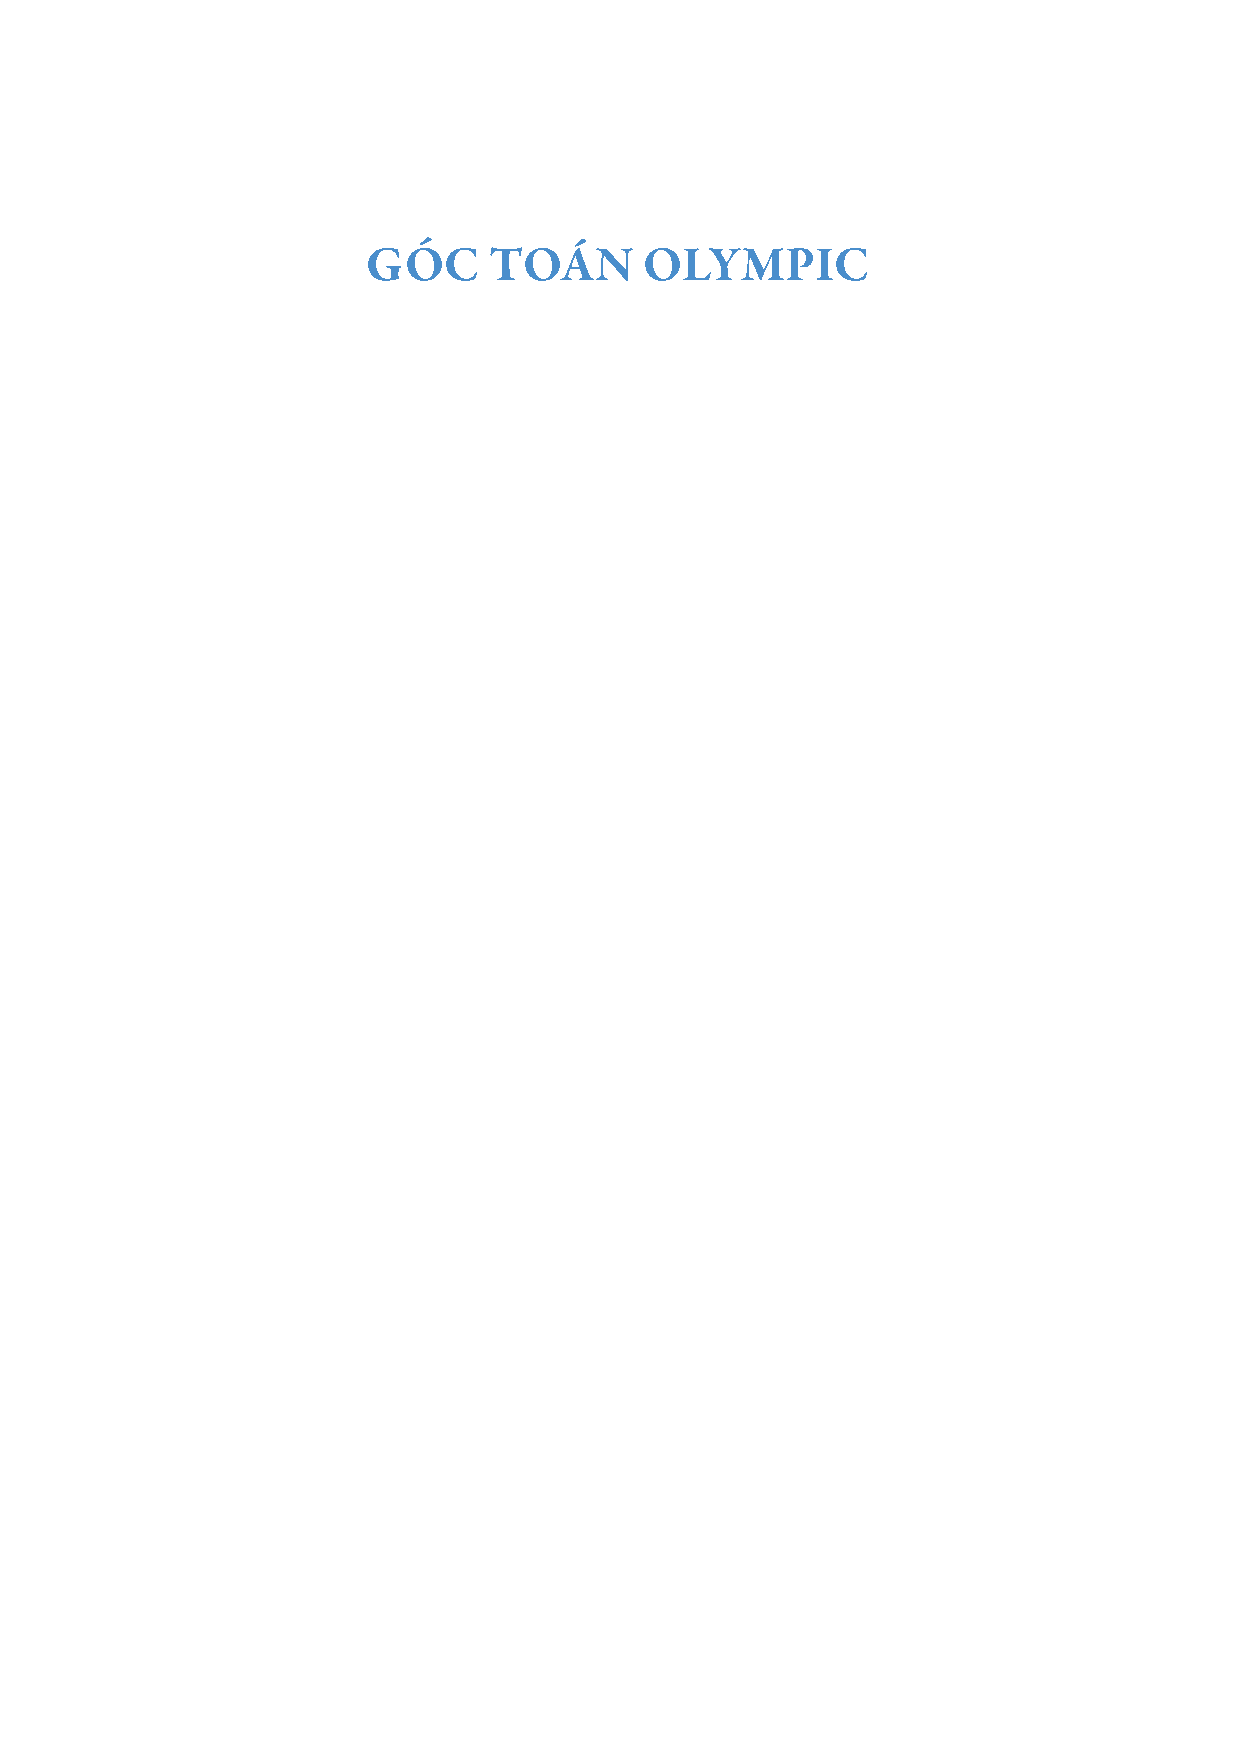
\includegraphics[scale=1]{../tieude1.pdf}}}
\centering
\endgroup
\vspace*{10pt}

\begin{multicols}{2}
	Trong phần đầu chuyên mục, chúng tôi sẽ trình bày lời giải của các bài toán trong kỳ thi Olympic Toán học trẻ của Ba Lan năm $2022$  đăng trong số báo $7-8/2022$. 
	\begin{figure}[H]
		\centering
		\vspace*{-5pt}
		\captionsetup{labelformat= empty, justification=centering}
		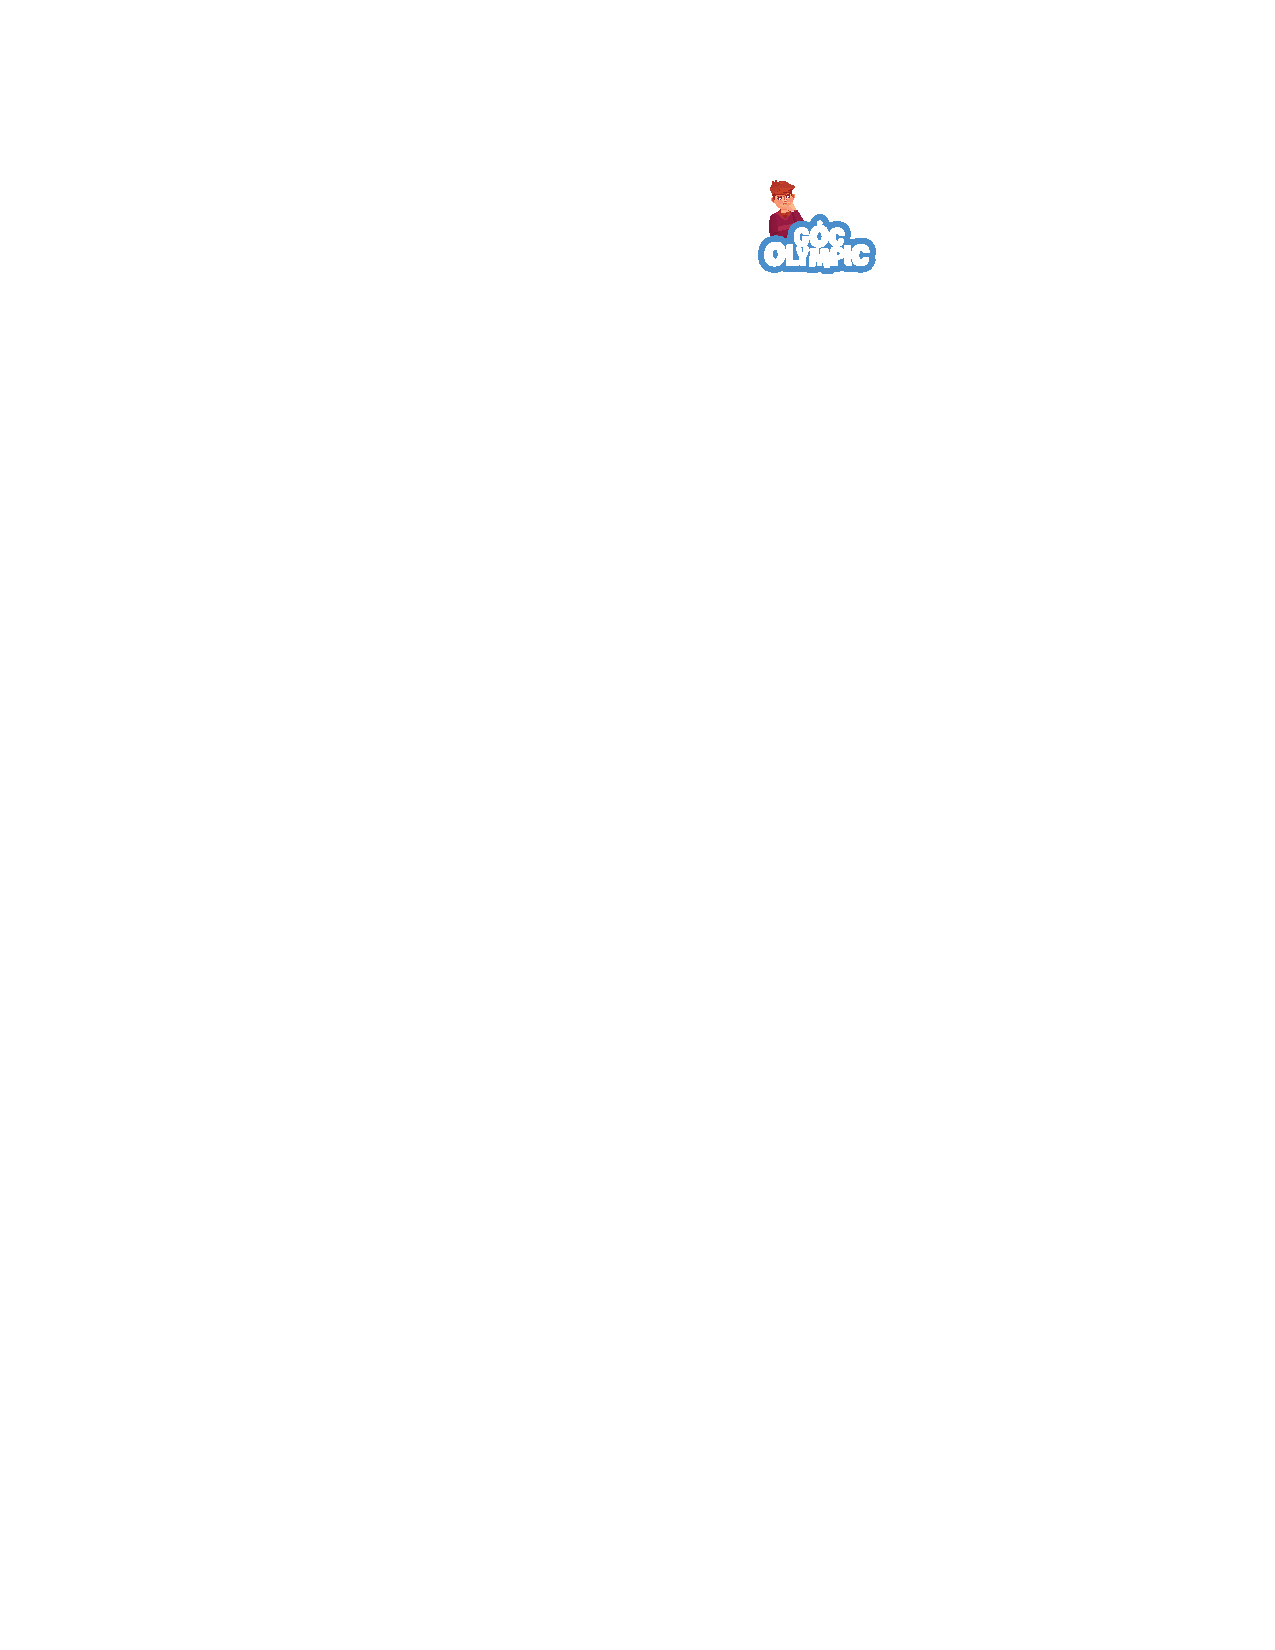
\includegraphics[width=1\linewidth]{gocolympic}
		\vspace*{-10pt}
	\end{figure}
	{\bf\color{cackithi} OC$\pmb{16.}$}  Trong lớp của Marek có $17$ học sinh và tất cả đều làm một bài kiểm tra. Biết rằng điểm của Marek cao hơn $17$ điểm so với điểm trung bình của các học sinh còn lại trong lớp. Hỏi điểm của Marek cao hơn điểm trung bình của cả lớp là bao nhiêu?
	\vskip 0.1cm
	\textit{Lời giải.} Ta gọi điểm của Marek là $m$. Khi đó, điểm trung bình  của tất cả  $16$ học sinh còn lại là $m - 17$, do đó tổng điểm của họ là $16(m - 17)$. Như vậy tổng điểm thu được của cả lớp bằng
	\begin{align*}
		16(m - 17) + m& =  17m - 16\times 17 \\
		&= 17(m - 16).
	\end{align*}
	Do đó ta suy ra điểm trung bình của cả lớp là $\dfrac{17(m - 16)}{17}= m - 16$. Như vậy điểm của Marek cao hơn $16$ điểm so với điểm trung bình của cả lớp. 
	\vskip 0.1cm
	Ta cũng có thể giải cách thứ hai như sau. Nếu Marek chia bớt cho mỗi bạn còn lại trong lớp $1$ điểm thì điểm trung bình của $16$ bạn còn lại sẽ tăng lên $1$ điểm còn điểm trung bình của cả lớp không thay đổi. Trong khi đó điểm của Marek, sau khi giảm đi $16$ điểm,  đúng bằng điểm trung bình của $16$ bạn còn lại, sau khi mỗi bạn nhận thêm $1$ điểm. Như vậy giá trị này cũng chính là điểm trung bình của cả lớp. Tức là điểm trung bình của cả lớp kém Marek $16$ điểm.    
	\vskip 0.1cm
	{\bf\color{cackithi} OC$\pmb{17.}$} Giả sử mỗi ô vuông trong bảng dưới đây được điền một số nguyên dương từ $1$ đến $17$ sao cho:
	\vskip 0.1cm
	-- Các số được điền đôi một phân biệt;
	\vskip 0.1cm
	-- Tổng của các số trong mỗi cột đều bằng nhau và tổng các số ở hàng trên cùng gấp đôi tổng các số ở hàng dưới cùng.
	\vskip 0.1cm
	Hỏi trong các số từ $1$ đến $17$, số nào không được điền vào bảng? Vì sao?
	\begin{figure}[H]
		\vspace*{-5pt}
		\centering
		\begin{tikzpicture}[scale=0.87]
			\draw[cackithi] (0,0) grid (8,2);
		\end{tikzpicture}
		\vspace*{-5pt}
	\end{figure}
	\textit{Lời giải.} Gọi $n$ là số không xuất hiện trong bảng. Khi đó tổng các số trong bảng là $1+2+ \cdots 17 -n= 153-n.$ Từ giả thiết, ta suy ra tổng các số trong bảng phải chia hết cho $3$ và $8$. Như vậy $(153-n)$ chia hết cho $24$. Chỉ có duy nhất một giá trị $n=9$ thỏa mãn.  
	\vskip 0.1cm
	Có nhiều cách để điền các số $1\le n \le 17$, $n\ne 9$ vào bảng thỏa mãn tất cả các điều kiện trong đầu bài. Chẳng hạn, ta điền như sau:
	\begin{figure}[H]
		\vspace*{-5pt}
		\centering
		\begin{tikzpicture}[scale=0.87]
			\draw[cackithi] (0,0) grid (8,2);
			\node at (0.5,0.5){$1$};
			\node at (1.5,0.5){$2$};
			\node at (2.5,0.5){$15$};
			\node at (3.5,0.5){$4$};
			\node at (4.5,0.5){$5$};
			\node at (5.5,0.5){$6$};
			\node at (6.5,0.5){$7$};
			\node at (7.5,0.5){$8$};
			\node at (0.5,1.5){$17$};
			\node at (1.5,1.5){$16$};
			\node at (2.5,1.5){$3$};
			\node at (3.5,1.5){$14$};
			\node at (4.5,1.5){$13$};
			\node at (5.5,1.5){$12$};
			\node at (6.5,1.5){$11$};
			\node at (7.5,1.5){$10$};
		\end{tikzpicture}
		\vspace*{-5pt}
	\end{figure}
	{\bf\color{cackithi} OC$\pmb{18.}$} Các điểm $K, L, M$ lần lượt nằm trên các cạnh $BC, CA, AB$ của tam giác đều
	$ABC$ và thỏa mãn các điều kiện sau:
	\begin{align*}
		KM = LM, \angle KML = 90^\circ \ \text{\color{black}và} \ AM = BK.
	\end{align*}
	Chứng minh rằng $\angle CKL = 90^\circ.$
	\vskip 0.1cm
	\columnbreak
	{\bf\color{cackithi} Lời giải.} 
	\begin{figure}[H]
		\centering
		\vspace*{-5pt}
		\captionsetup{labelformat= empty, justification=centering}
			\begin{tikzpicture}[cackithi,scale=1.2]
				\draw[fill=lightgray] (2.459119433858577,0.33899142094742796) -- (2.120128012911149,0.40652583282801863) -- (2.052593601030558,0.06753441188059066) -- (2.391585021977986,0) -- cycle; 
				\draw [] (0,0)-- (4,0);
				\draw [] (4,0)-- (2,3.4641016151377553);
				\draw [] (2,3.4641016151377553)-- (0,0);
				\draw [] (2.391585021977986,0)-- (2.8042074890110076,2.0711733843433016);
				\draw [] (2.4940559957207333,1.0147377863273366) -- (2.6858185017335243,0.9765345538439683);
				\draw [] (2.5099740092554703,1.0946388304993333) -- (2.7017365152682618,1.056435598015965);
				\draw [] (0.24670542797194478,0.42730633575043236)-- (2.391585021977986,0);
				\draw [] (1.2982963191306511,0.31749342764898086) -- (1.2600930866472826,0.12573092163618976);
				\draw [] (1.378197363302648,0.3015754141142439) -- (1.3399941308192795,0.10981290810145276);
				\draw [dashed] (0.8042074890110077,1.3929282307944546)-- (2.8042074890110076,2.0711733843433016);
				\draw [dashed] (1.7342316770218398,1.811554657546376) -- (1.7970279601909558,1.6263818396042484);
				\draw [dashed] (1.8113870178310594,1.8377197755335073) -- (1.8741833010001756,1.6525469575913798);
				\draw [dashed] (0.8042074890110077,1.3929282307944546)-- (2.391585021977986,0);
				\draw [dashed] (1.631760703279094,0.7968168712190403) -- (1.502794480435417,0.6498472857602803);
				\draw [dashed] (1.6929980305535766,0.7430809450341749) -- (1.5640318077098996,0.5961113595754148);
				\draw [] (0,0)-- (2.391585021977986,0);
				\draw [] (1.1957925109889933,0.09776546640363895) -- (1.1957925109889933,-0.09776546640363895);
				\draw [] (2,3.4641016151377553)-- (0.8042074890110077,1.3929282307944546);
				\draw [] (1.4867711220238906,2.379632189764285) -- (1.3174363669871194,2.477397656167924);
				\draw [] (2.8042074890110076,2.0711733843433016)-- (4,0);
				\draw [] (3.4867711220238897,1.0844694253734704) -- (3.3174363669871187,0.9867039589698313);
					\draw [fill=white] (0,0) circle (1.5pt);
					\draw[] (-0.23217938838527713,-0.22874971994316104) node {$A$};
					\draw [fill=white] (4,0) circle (1.5pt);
					\draw[] (4.2813263105827275,-0.19616123114194808) node {$B$};
					\draw [fill=white] (2,3.4641016151377553) circle (1.5pt);
					\draw[] (1.9349551168953893,3.9588710910127074) node {$C$};
					\draw [fill=white] (2.391585021977986,0) circle (1.5pt);
					\draw[] (2.391193960112372,-0.2613382087443741) node {$M$};
					\draw [fill=white] (2.8042074890110076,2.0711733843433016) circle (1.5pt);
					\draw[] (2.9940810029348133,2.427212117355697) node {$K$};
					\draw [fill=white] (0.24670542797194478,0.42730633575043236) circle (1.5pt);
					\draw[] (-0.069236944379212,0.765199188493835) node {$L$};
					\draw [fill=white] (0.8042074890110077,1.3929282307944546) circle (1.5pt);
					\draw[] (0.5010616096420161,1.8406193189338635) node {$N$};
			\end{tikzpicture}
		\vspace*{-10pt}
	\end{figure}
	Lấy điểm $N$ trên cạnh $AC$ sao cho $AM = BK = CN$ như hình bên trên. Từ đó ta có $BM = CK = AN$, vì vậy các tam giác $AMN, BKM, CNK$ bằng nhau (cạnh--góc--cạnh) và do đó tam giác $KMN$ đều. 
	\vskip 0.1cm
	Từ việc tam giác $KMN$ đều, kết hợp với giả thiết $KM=LM$ ta suy ra tam giác $NML$ cân tại $M$. Hơn nữa ta có $\angle LMN=90^{\circ}-60^{\circ}=30^{\circ}$. Vì vậy, $\angle NLM = \dfrac{180^{\circ}-30^{\circ}}{2}=75^{\circ}$. Ta nhận được
	$\angle CLK= \angle NLM - \angle KLM= 75^{\circ}-45^{\circ}= 30^{\circ}$. Từ đây ta suy ra $\angle CKL = 180^{\circ}-30^{\circ}-60^{\circ}=90^{\circ}$.   
	\vskip 0.1cm
	{\bf\color{cackithi} Nhận xét.} Giả thiết $\angle KML =90^{\circ}$ có thể thay bằng điều kiện yếu hơn là $\angle KML \neq 60^{\circ}.$ Thực vậy, khi đó $L\neq N$ và vẫn lý luận như trên ta cũng nhận được tam giác $NML$ cân tại $M.$ Do đó
	\begin{align*}
		\angle CLK\!&=\! \angle NLM - \angle KLM\\
		&= \!\frac{180^{\circ}\!\!-\!\!\angle NML}{2} \!\!-\!\! \frac{180^{\circ}\!\!-\!\!\angle NML \!-\! 60^{\circ}}{2}\\
		&=\!30^{\circ}.
	\end{align*}
	Như vậy ta vẫn nhận được $\angle CKL =90^{\circ}.$  
	\vskip 0.1cm
	Trong phần cuối của chuyên mục kỳ này, chúng tôi sẽ giới thiệu với bạn đọc ba bài toán trong kỳ thi Olympic Toán học Trẻ của Canada năm học $2022$. Các bài toán này phù hợp với trình độ học sinh năm cuối cấp Trung học cơ sở.
	\vskip 0.1cm
	{\bf\color{cackithi} OC$\pmb{25.}$} Cho $ABC$ là tam giác nhọn nội tiếp đường tròn $\Gamma.$ Đường thẳng qua $A$ vuông góc với $BC$ cắt $\Gamma$ tại $D,$ và đường thẳng qua $B$ vuông góc với $AC$ cắt $\Gamma$ tại $E.$ Chứng minh rằng nếu $AB = DE$, thì $\angle ACB = 60^{\circ}$.
	\vskip 0.1cm
	{\bf\color{cackithi} OC$\pmb{26.}$} Giả sử bạn có vô hạn các hình chữ $T$ (bao gồm bốn hình vuông cạnh
	$1$) như trong hình vẽ, và một bảng ô vuông cỡ $n \times n.$ Bạn được phép đặt một số hình trên bảng (có thể xoay chúng), miễn là không có hai hình nào chồng lên nhau và không có hình nào vượt ra khỏi bảng.
	\vskip 0.1cm
	Với những giá trị nào của $n$ thì bạn có thể phủ toàn bộ bảng?
	\begin{figure}[H]
		\centering
		\vspace*{-5pt}
		\captionsetup{labelformat= empty, justification=centering}
		\begin{tikzpicture}[cackithi]
			\draw (0,0) grid (3,1);
			\draw (1,1) grid (2,2);
		\end{tikzpicture}
		\vspace*{-10pt}
	\end{figure}
	{\bf\color{cackithi} OC$\pmb{27.}$} Giả sử rằng các số thực $a$ và $b$ thỏa mãn
	\begin{align*}
		ab+ \sqrt{ab+1} +\sqrt{a^2+b}\ \sqrt{b^2+a}=0.
	\end{align*}
	Tìm giá trị của biểu thức
	\begin{align*}
		S=a\sqrt{b^2+a} + b\sqrt{a^2+b}.
	\end{align*}
\end{multicols}